Before arriving to its final form, several designs for the PD-SD were considered. Here are listed the various alternatives weighed:

\paragraph{Humanoid} The most natural form an assitive robot can take to replace a person in home chores is that of another, since homes are designed to be controlled and navigated by humans. \\

Therefore a humanoid robot was the inmediate answer: its degrees of freedom would enable it to carry out the same tasks as their human counterparts, it would have the right size to be able to handle objects placed in high furniture and it would have a form that would generate an emotional response from the user.\\

However, the humanoid has one major disadvantage, control. While two-legged robots do exist, as seen previously with Honda's ASIMO, they are very unstable and require active control algorithims to balance it. \\

To make the droid stable even when unpowered and to simplify the algorithims the legs were replaced by a wheeled base. This also had the side effect of reducing the cost, since each wheel would be driven by one motor to provide a differential drive, instead of a total of twelve motors for a pair of full human like legs, with three to simulate the hip joint, one for the knee and two more for the ankle, per leg.\\


\paragraph{Four wheels} The first wheeled base design envisaged four wheels in order to keep it stable, each with its own motor. However, the design is redundant, as a two-wheeled base with a caster at the rear end is equally stable but reduces the number of active wheels. This decreases the price, the power consumption, frees up two pins on the micro controller and reduces the length of the code, while remaining suitable to support the robot.


\paragraph{Exoskeleton} One of the first designs is shown in Figure \ref{exoskeleton}. It featured a robot with an exoskeleton and a central beam. This version granted different levels into which the various components could be placed while hiding the cables inside. \\

	\begin{figure}[H]
			\centering
			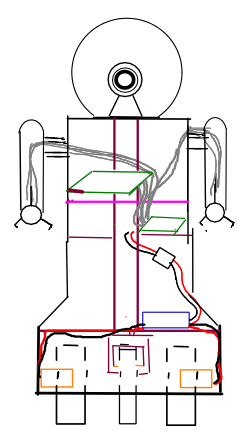
\includegraphics[scale=0.4]{images/Diagrams/exoskeleton}
			\caption{}
			\label{exoskeleton}
	\end{figure}
	\bigskip

However, it provided very little stability and a design with a more human-like skeleton was chosen.\\


\paragraph{Arm designs}
-> gripper vs hand
 -> Pictures of different designs -> Better because of firmer grip, less torque on plastic... 
\\	






5 dof (4+1) ensure redundancy and posssibility of linear movement for some detailed tasks

denavit hartenberg for arms

